%% ====================================================================
\section{Implementation}
\label{section:implementation}


This section describes in great details how we connected a set of
virtual machines (VMs) running on Knox, a cloud cluster in Sweden, to
another set of VMs running on ePouta, a cloud cluster in Finland. The
two clusters are managed by
\href{http://docs.openstack.org/liberty/install-guide-ubuntu/}{Openstack
  Liberty}.

We start with the low-level component. There is a 1GB/s fiber-link
between Knox and ePouta with a dedicated network. This means that the
link might be shared, but only the VMs on that network can communicate
through it. This security is provided by VLAN encapsulation. In our
case, the VLAN tag is 1203.

We use the following range of IPs: \ip{10.101.0.0/16} for network
communication between the VMs. We split the address range in two
disjoint parts. For that, we use the third number of the
\ip{10.101.0.0/16} CIDR. The VMs in ePouta will have an IP where the
third number starts in binary notation with a \texttt{0}, while, for the
VMs in Knox, the third number will start with a \texttt{1}. The
exception is the virtual router.

The network settings use the following components:
\begin{itemize}
\item a Virtual Router on Knox (with IP: \ip{10.101.0.1/16})
\item a DHCP server on Knox (with IP: \ip{10.101.128.0/16})
\item a DHCP server on ePouta (with IP: \ip{10.101.0.3/16})
\item the Neutron linuxbridges plugin (on Knox) with VLAN capabilities
\item a set of VMs on ePouta (with IPs from \ip{10.101.0.4/16} to
  \ip{10.101.127.255/16})
\item a set of VMs on Knox (with IPs from \ip{10.101.128.1/16} to
  \ip{10.101.128.254/16})
\end{itemize}

The DHCP server on Knox (resp. ePouta) provides network information for
the VMs on Knox (resp. ePouta).

It is necessary to adjust the network settings in ePouta accordingly.

\codeblock{adjust-epouta.sh}

Note that we also adjusted the DNS setting. In the namespace related
to the DHCP server lies a \texttt{dnsmasq} process, which accepts DNS
queries and either answers them from a small, local, cache or forwards
them to a real, recursive, DNS server. Therefore, we make the VMs DNS
queries point to \ip{10.101.128.0}.

\subsection{The Virtual Router and DHCP server, \emph{on  Knox}}
\label{section:virtual:router}
\label{section:dhcp:server:knox}

Openstack uses the network namespace capabilities of the Linux kernel,
in order to isolate routes, firewall rules and interfaces from the
root namespace. This is where the virtual router and the dhcp server
live, each in its own namespace. Note that we are using
\href{http://docs.openstack.org/liberty/install-guide-ubuntu/}{Openstack
  Liberty} on Knox, and that the naming convention is such that
network components (often) start with \texttt{q}. This is for
historical reasons: \emph{Neutron} used to be called
\emph{Quantum}. We use \texttt{\textless{}...\textgreater{}} to denote
a \emph{universally unique identifier} (such as
\texttt{1a6abf7e-f927-4598-9a6c-c4311e685e52}).

The following commands run on the Knox \texttt{controller}.

\codeblock{ip-netns.sh}

The neutron plugin creates veth pairs, where one end is moved to a
network namespace, and the other end is still in the root namespace.
The end in the router namespace is of the form
\texttt{qr-\textless{}...\textgreater{}} and the one in the dhcp
namespace is of the form \texttt{ns-\textless{}...\textgreater{}}. The
other end of the veth pairs, in the root namespace, is added to a
linux bridge. Openstack creates a linux bridge per project.

Moreover, the plugin makes sure that the outgoing interface, of the
physical host, uses the VLAN tag 1203, and is also added to that same
bridge, therefore providing connectivity and security to the router
(over that VLAN).

The dhcp namespace isolates a \texttt{dnsmasq} process, while the
other
namespace isolates routes and IPtables rules for the virtual router.

%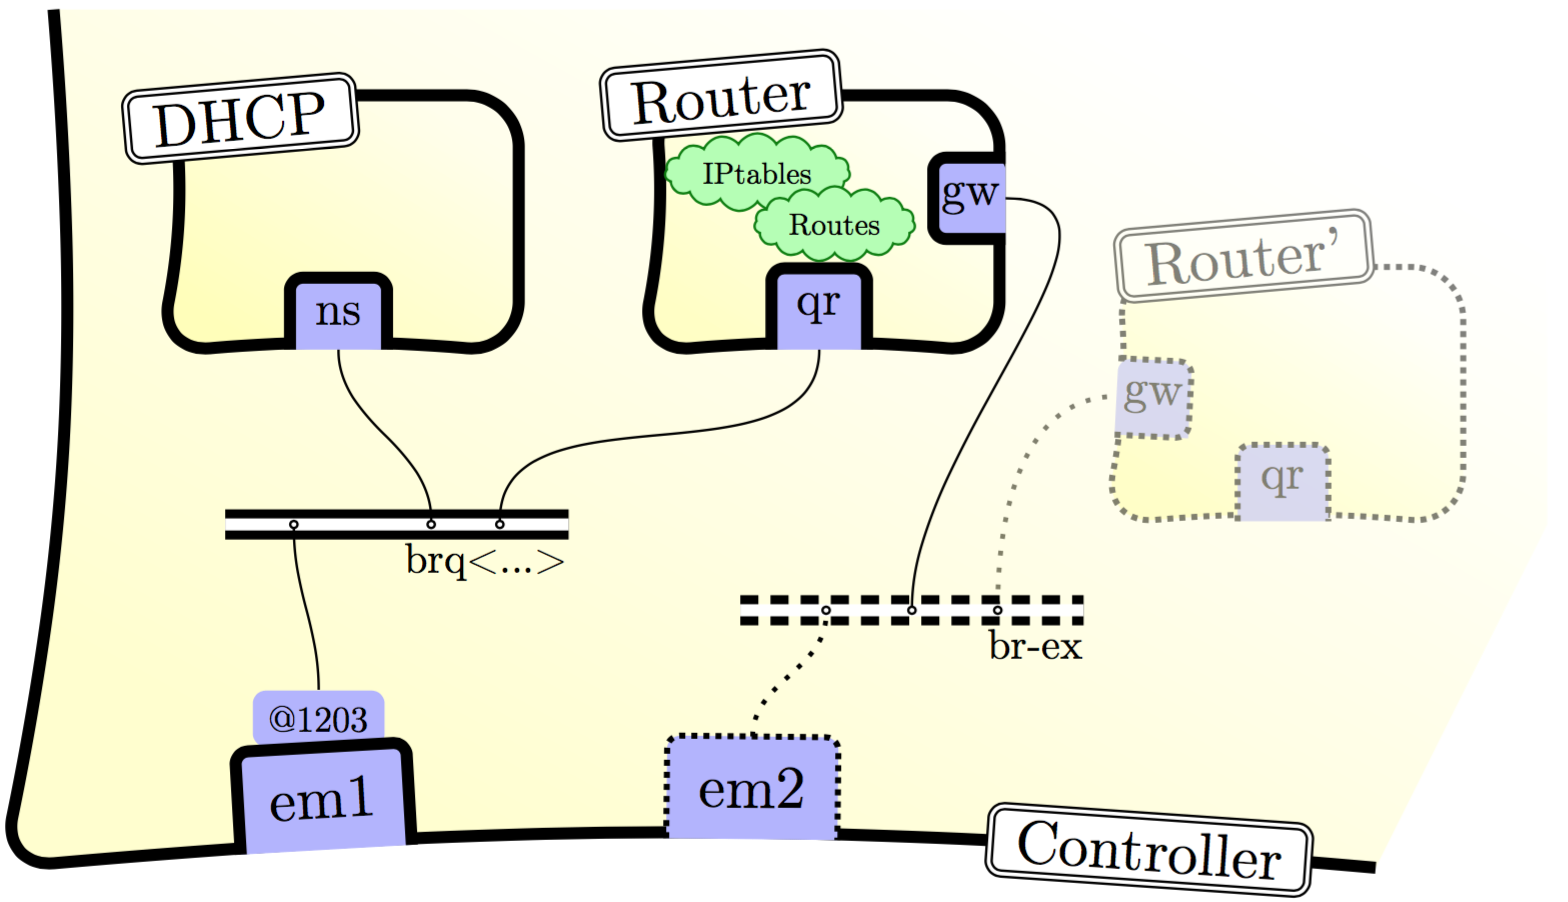
\includegraphics{./img/controller.jpeg}

The following openstack commands create the necessary underlying
components on the Knox \texttt{controller} for providing connectivity
between the different VMs, either in Knox or in ePouta. The components
are a network namespace, a bridge, and a veth pair that is dedicated
for the 10.101.0.0/16 network.

\codeblock{neutron-commands-knox.sh}

Both the virtual router and the DHCP server are connected to the root
namespace via 2 tap interfaces, added to a common bridge. Openstack
also created a VLAN interface (with 1203) on that bridge for the
\ip{10.101.0.0/16} network.

\codeblock{bridge.sh}

\begin{quote}
  Note: We think we found a problem with MAC addresses on the linux
  bridge in Ubuntu: The tap interface connected to the virtual router
  is learned on the wrong port of the bridge. Moreover, the MAC
  address of the bridge itself is by construction to lowest one of all
  its interfaces, unless its MAC address is fixed at
  creation. Updating the openstack plugin for fixing the bridge's MAC
  address was not a solution in mind. Instead, we opted for the
  following quickfix: We disabled the MAC learning algorithm of the
  bridge, and made it behave like a hub (and not a virtual switch). We
  don't recall that it was necessary on CentOS.

  The following command (as root) provides a solution (albeit
  non-optimal):

  \codeblock{bridge-ageing.sh}
\end{quote}

\subsection{External connectivity for the VMs}
\label{section:external:connectivity}

All VMs have a default route to the virtual router. Therefore,
external connectivity is adjusted in the virtual router's namespace
(on Knox).

Openstack usually creates a veth pair, where one end is a
\texttt{gateway} interface added to the virtual router, and the router
translates the source address (\emph{source NATing} or \emph{SNAT}),
using IPTables, for outgoing traffic over that interface. Traffic to
the \ip{10.101.0.0/16} network is routed through the
\texttt{qr-\textless{}...\textgreater{}} interface, and all other
traffic is routed through the gateway interface.

The other end of the veth pair is still in the root namespace, and is
added to an \emph{external} bridge, which already forwards traffic to
the host's external interface. That way, all virtual routers have
external connectivity.

However, in our case, we did not need to use this (classic) openstack
setup. We instead used a single veth pair (denoted \texttt{gw\
  \textless{}-\textgreater{}\ mm}), along with a \emph{fake
  external/local} network \texttt{10.5.0.0/24}. The \texttt{gw} end
belongs to the virtual router and has the IP \texttt{10.5.0.2/24},
while \texttt{mm} has \texttt{10.5.0.1/24}.

On the controller:

\codeblock{gw-mm.sh}

Inside the Virtual router:

\codeblock{gw-mm-vr.sh}

The routes in the Virtual Router are so far:

\codeblock{routes-vr.sh}

We chose to not give a full external connectivity to the VMs. We do
not have a \texttt{default} route in the routing table of the virtual
router. Instead, we only added a few extra routes as follows:

\codeblock{routes-vr-extra.sh}

Finally, for external connectivity, it is necessary to \emph{source
  NAT} the traffic coming out of the virtual router.

\codeblock{snat.sh}

\subsection{VM connectivity on the compute nodes}
\label{section:connectivity:compute:nodes}

On each compute node, a bridge is created (also per project), along
with an interface with VLAN tag 1203. A veth pair's end is added to
the bridge, while to other end is used by a VM, as its internal
interface.

A kernel setting is used to force IPtables to filter traffic on the
bridge. This is the way Openstack enforces security groups and in
particular ensures some address spoofing protections. These rules can
be slightly manipulated by updating the neutron port settings.

\codeblock{bridge-cn.sh}

%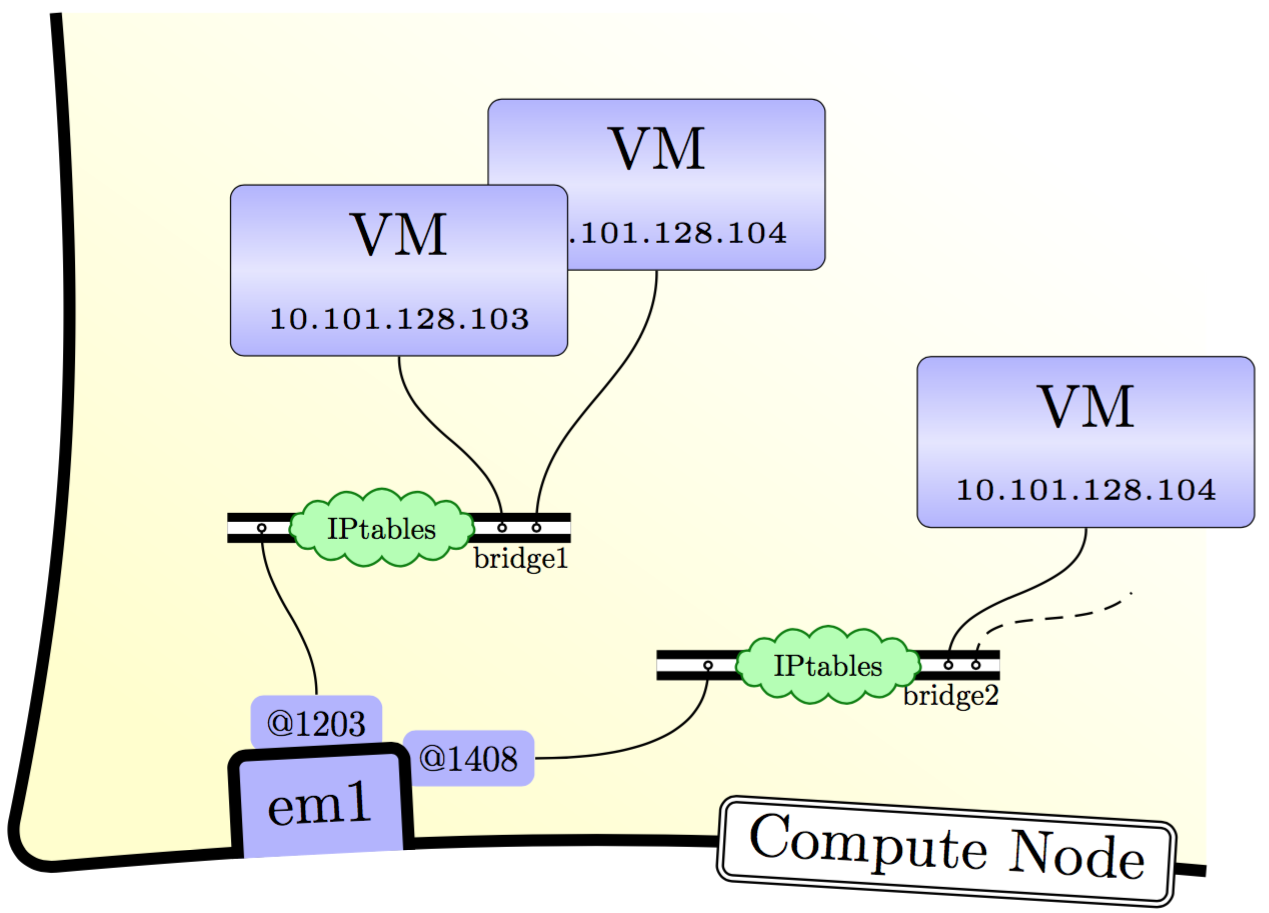
\includegraphics{./img/compute-node.jpeg}

Let us describe in greater details how the security rules are
implemented. This is relevant to understand pitfalls in connecting the
VMs from different clouds together.

If we display the \texttt{FORWARD} chain, we see the openstack add a
``relay'' chain, named \texttt{neutron-linuxbri-FORWARD}.

\codeblock{iptables-forward.sh}

All rules are now in that relay chain. If the traffic, whether inwards
or outwards, goes through the VM interface, via the tap interfaces, it
is redirected to the security group chain.

\codeblock{iptables-forward-neutron.sh}

The security group chain gathered all incoming and outgoing traffic
from the VMs. Surprisingly, that chain now forks and redirects the
traffic to an \emph{incoming} or another \emph{outgoing} chain. If
those latter chains do not filter the traffic, the packets are then
accepted.

\codeblock{iptables-sg-chain.sh}

Let us now inspect the outgoing chain onto a particular VM (Note the
name starting with \emph{neutron-linuxbri-\textbf{o}}). It starts by
allowing traffic from the DHCP client (by returning to the previous
chain, wich accepts the traffic).

\codeblock{iptables-neutron-sg-input.sh}

Otherwise, it jumps to a \emph{source chain} (which name starts with \emph{neutron-linuxbri-\textbf{s}}).

\codeblock{iptables-neutron-sg-source.sh}

The source chain filters out traffic that is not the proper pair of IP
and MAC address related to that VM. This is important since a VM
cannot then simply add a network or an interface and connect through
it. In the hypothetical scenario where that VM creates a bridge, the
MAC address of the bridge might flicker between the ones from the
added interfaces. Moreover, in another scenario where the VM network
is augmented with another local network, say \ip{192.168.0.0/24}, the
traffic would be filtered by the source chain. This is relevant in
case we want to implement on openstack installation inside VMs (such
as Mosler, or the so-called \emph{Triple-O}, Openstack on Openstack).

Back to the outgoing chain, after checking the allowed IP/MAC pair
(which can be updated through some neutron commands), it checks for
established connections, or drops them if they are invalid. In other
cases, the filtering continues onto a \emph{fallback chain} which
simply drops that traffic.

\codeblock{iptables-neutron-sg-output.sh}

Finally, we observe that the openstack security rules, which we added
in neutron, end up in the \emph{incoming chain} (which name starts
with \emph{neutron-linuxbri-\textbf{i}}). The DHCP traffic is allowed,
along with \texttt{ping} and tcp traffic (on all ports), from the IP
range \ip{10.101.0.0/16}. Some specific neutron commands can allow
other network ranges, and this is where the rules would appear.

\codeblock{iptables-neutron-sg-input-2.sh}

In case the above ping and tcp rules were absent, the traffic is then
accepted if it comes from another VM on the network. This is
implemented with IPset.

\codeblock{iptables-neutron-ipset.sh}

Notice here that the set contains the IP of the machines that were
booted on Knox, and not ePouta. We would have to update the IPset, or
update the plugin itself to automatically include the other VMs across
borders. It was not necessary since we had the `All tcp ports' rule
already in place.

\section{Remarks}\label{remarks}

Broadcast traffic is still forwarded to all interfaces on VLAN 1203
and therefore to all VMs. An improvment would be to use OpenVSwitch to
learn about MAC addresses and skip physical nodes that don't host any
VMs on that project. That will improve East-West traffic. An
alternative is to distribute the router using DVR (not available when
using the Linux Bridge mechanism).
